% ЕМТ 2025, VII клас — точен LaTeX препис от официалните файлове в Klasirane.com.
% Условия: https://klasirane.com/api/competitions/EMT/All/2025/7%20%D0%BA%D0%BB/probs
% SHA-256 (условия): 15c4f0841e55d81cd961b4411be2cc98ccdaceee4505dfb140ad4b762fee7fc0
% Решения: https://klasirane.com/api/competitions/EMT/All/2025/7%20%D0%BA%D0%BB/sol
% SHA-256 (решения): 325b8832092f13d590c7545d9601c86ba53643da46d1c89437e1cbdaabe29564
% Точковите оценки, правописът и формулировките са запазени от източника.

Задача 7.1. а) Пресметнете стойността на израза

$$A=1^2-2^2+3^2-4^2+\cdots+23^2-24^2+2025.$$

б) Ако

$$\dfrac{48^n:3^{n-2}-4^{2n}}{(4^n+1)(16^n-4^n+1)-(8^n-1)^2}=2^k,$$

където $k$ е най-големият прост делител на $A$, намерете $n$.

Решение. а) Намираме

$$A=(1-2)(1+2)+(3-4)(3+4)+\cdots+(23-24)(23+24)+2025=$$

$$=-3-7-11-\cdots-47+2025=6\cdot(-50)+2025=1725.$$

(2 точки)

б) Числителят на израза е равен на

$$48^n:3^{n-2}-4^{2n}=2^{4n}\cdot3^n:3^{n-2}-2^{4n}=2^{4n}(3^2-1)=8\cdot2^{4n}=2^{4n+3}.$$

Знаменателят на израза е равен на

$$(4^n+1)(16^n-4^n+1)-(8^n-1)^2=4^{3n}+1-8^{2n}+2\cdot8^n-1=2^{6n}-2^{6n}+2^{3n+1}=2^{3n+1}.$$

Тогава лявата страна на равенството е

$$2^{4n+3}:2^{3n+1}=2^{n+2}.$$

(3 точки)

Тъй като $1725=3\cdot5^2\cdot23$, то $k=23$. Получаваме $n+2=23$, т.е. $n=21$.

(1 точка)

Задача 7.2. Участък има форма на кръг с център $O$ и радиус 14 m. Собственикът на участъка заградил правоъгълен двор $ABCD$ с висока ограда, като центърът $O$ е върху страната $AB$. Оказало се, че $OA=3,5$ m, $AB=4\cdot AD$ и

$$AD^2+DO^2=OB^2.$$

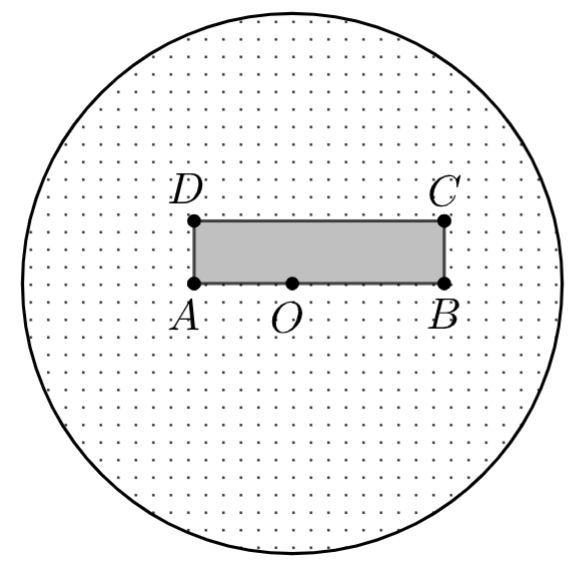
\includegraphics[max width=0.38\textwidth, alt={Кръглият участък и правоъгълният двор ABCD с център O върху AB}, center]{assets/7-2-plot.jpg}

а) Намерете обиколката на $ABCD$.

б) Собственикът превърнал останалата част от участъка в тревна площ, засята с ливадни треви. В центъра $O$ е прикрепено 7-метрово въже и на другия му край е вързана коза, която се намира извън $ABCD$ и не може да прескочи оградата. Пресметнете с точност до цяло число най-много какъв процент от тревната площ може да е достъпна за козата $(\pi\approx\dfrac{22}{7})$.

Решение. а) Нека $AD=x$ m. Тогава $AB=4x$ и $OB=4x-3,5$. Според теоремата на Питагор, приложена за правоъгълния триъгълник $AOD$,

$$OD^2=x^2+3,5^2.$$

От условието следва, че

$$x^2+(x^2+3,5^2)=(4x-3,5)^2\Longleftrightarrow x^2=2x$$

и тъй като $x\ne0$, получаваме $x=2$. Тогава $AB=8$ m и $P_{ABCD}=20$ m.

(3 точки)

б) Тревната площ е $14^2\pi-2\cdot8\approx616-16=600$ m$^2$. Достъпната за козата площ $S$ се състои от полукръг с радиус 7 m и четвъртинки от кръгове с радиуси 3,5 m, 2,5 m, 1,5 m, 0,5 m.

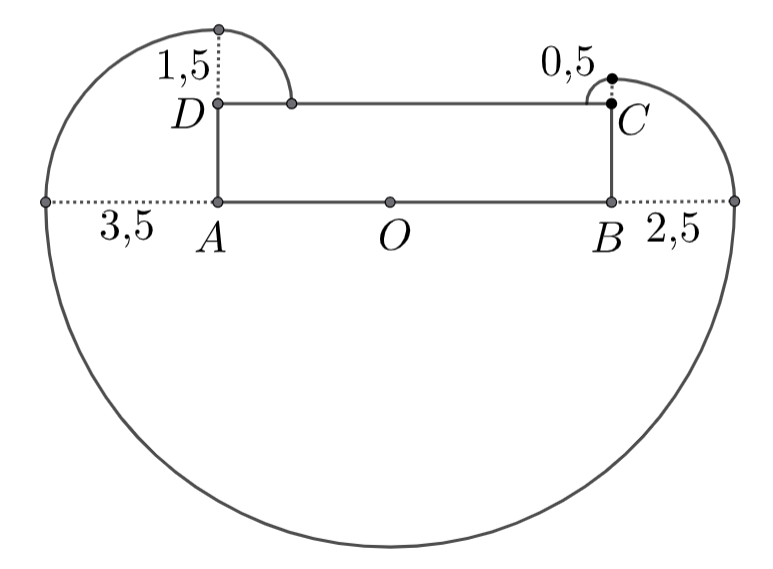
\includegraphics[max width=0.58\textwidth, alt={Достъпната за козата площ около правоъгълния двор}, center]{assets/7-2-goat-reach.png}

Тогава

$$S=\dfrac{1}{2}\cdot49\pi+\dfrac{\pi}{4}(3,5^2+2,5^2+1,5^2+0,5^2)=\dfrac{119}{4}\pi\approx93,5\text{ m}^2.$$

От

$$\dfrac{93,5}{600}=15\dfrac{7}{12}\%\approx16\%$$

следва, че най-много 16% от тревната площ е достъпна за козата.

(3 точки)

Задача 7.3. Естествените числа $a$ и $b$ са такива, че стойността на всеки от изразите

$$\dfrac{a^2+3^b}{4}\quad\text{и}\quad\dfrac{a^3+4^b}{5}$$

е естествено число. Да се докаже, че стойността на израза

$$\dfrac{(a+b)^2-(a-1)^2-(b+1)^2}{40}$$

е цяло число.

Решение. Възможните остатъци на $a^2$ при деление на 4 са 0 и 1 (от $a\equiv0,1,2,3\pmod{4}$ следва $a^2\equiv0,1,2^2,3^2\equiv0,1\pmod{4}$).

(1 точка)

Възможните остатъци на $3^b$ при деление на 4 са 3 и 1: (тъй като $3^{2k+1}=9^k\cdot3\equiv3\pmod{4}$, $3^{2k}=9^k\equiv1\pmod{4}$).

(1 точка)

Следователно сборът $a^2+3^b$ се дели на 4, само когато $a^2\equiv1\pmod{4}$ и $3^b\equiv3\pmod{4}$, което е изпълнено точно когато $a$ е нечетно число и $b$ е нечетно число.

(1 точка)

Тъй като $b=2k+1$, получаваме

$$4^b=4^{2k+1}=4\cdot16^k\equiv4\pmod{5}.$$

(1 точка)

Тъй като $a^3+4^b$ се дели на 5, то $a^3\equiv1\pmod{5}$. Това е възможно само при $a\equiv1\pmod{5}$ (тъй като $a^3\equiv0,1,2^3,3^3,4^3\equiv0,1,3,2,4\pmod{5}$).

(1 точка)

Следователно $(a-1)$ се дели на 5, а тъй като $a$ е нечетно число, $(a-1)$ се дели на 10. Остава да забележим, че

$$(a+b)^2-(a-1)^2-(b+1)^2=2(a-1)(b+1)$$

и полученото произведение се дели на 40.

(2 точки)

Забележка. Последния резултат може да получим и по друг начин. Тъй като $b=2k+1$ и $a-1=10m$, т.е. $a=10m+1$, то

$$(a+b)^2-(a-1)^2-(b+1)^2=(2k+10m+2)^2-(10m)^2-(2k+2)^2=40m(k+1),$$

откъдето директно следва, че даденият израз е цяло число.

Задача 7.4. Октаедърът на чертежа е съставен от две еднакви правилни четириъгълни пирамиди с обща основа. Стените на октаедъра са равнобедрени триъгълници, при които бедрата са по-големи от основата.

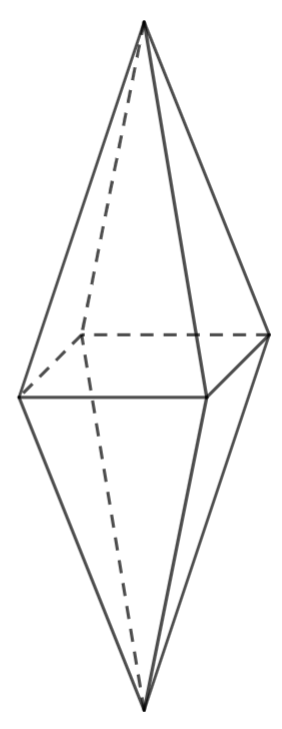
\includegraphics[max width=0.26\textwidth, alt={Октаедър от две еднакви правилни четириъгълни пирамиди}, center]{assets/7-4-octahedron.png}

На всяка от осемте стени на октаедъра е записано по едно от естествените числа от 1 до 8 (всяко число се използва точно веднъж).

За един ход можем да увеличим с 1 числата на две стени, които имат общ ръб.

Да се намери броят на различните начални разположения на числата, за които след краен брой ходове е възможно всички числа върху стените на октаедъра да станат равни.

Две разположения се считат за различни, ако едното не може да се получи от другото чрез завъртане на октаедъра.

Решение. Необходимост. Да оцветим стените на октаедъра шахматно в черно и бяло. Всеки ход увеличава с 1 сбора $S_b$ на числата на черните стени и сбора $S_w$ на числата на белите стени, т.е. разликата $S_b-S_w$ се запазва.

(1 точка)

Ако от дадено начално разположение на числата след краен брой ходове се получават равни числа на стените на октаедъра, то разликата $S_b-S_w=0$.

Тъй като в началото $S_b+S_w=1+2+\cdots+8=36$, необходимо условие да се получат равни числа на всички стени, е в началото

$$S_b=S_w=18.$$

(1 точка)

Без ограничение може да приемем, че на стената $ABE$ е записано числото 8. На трите едноцветни с $ABE$ стени трябва да се запишат числа със сбор 10:

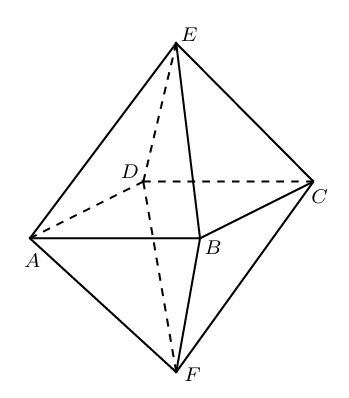
\includegraphics[max width=0.32\textwidth, alt={Означения A, B, C, D, E и F върху октаедъра}, center]{assets/7-4-labeled-octahedron.png}

$$1+2+7;\quad1+3+6,\quad1+4+5,\quad2+3+5,$$

а оставащите числа да се запишат на стените от другия цвят. Това може да стане по

$$4\cdot3!\cdot4!=576\text{ начина}.$$

(2 точки)

Достатъчност. Ще докажем, че от начално разположение на числата, което изпълнява условието $S_b=S_w$, може с краен брой ходове да стигнем до конфигурация с равни числа на стените.

Докато е възможно, на всеки ход избираме две съседни стени, на които са записани числа, по-малки от 8, и увеличаваме двете числа с 1.

Ако в даден момент няма две съседни стени с числа, по-малки от 8, то или на всички стени е записано числото 8 и задачата е решена, или съществува стена, на която е записано число $a<8$; да допуснем, че това е стената $BCE$. На съседните стени на $BCE$ е записано числото 8. Да забележим, че трите съседни стени на $BCE$ и стената $ADF$ са оцветени в един и същ цвят (нека е бял). Ако допуснем, че на стената $ADF$ е записано числото 8, то на всички бели стени има осмица. Понеже сборът на числата на черните и белите стени е един и същ, следва, че и на черните стени са записани осмици; противоречие. Следователно на стената $ADF$ е записано число $b<8$. Следователно на трите съседни стени на $ADF$ (които са черни) е записано числото 8. Сборът на числата на белите стени е $24+b$, сборът на числата на черните е $24+a$, следователно $a=b$.

За да изравним числата, забелязваме, че с 5 хода за стените

$$(BCE,BCF),\quad(BCE,ABE),\quad(ADF,ADE),\quad(ADF,ABF),\quad(DCF,DCE)$$

увеличаваме с 2 числата на стените $BCE$ и $ADF$, а числата на останалите стени увеличаваме с 1. Така разликата между шестте по-големи числа и двете по-малки се намалява с 1; продължавайки по този начин, ще направим числата на всички стени равни.

(3 точки)
